\chapter{Desenvolvimento}
\label{cap:desenvolvimento}

Nesta seção, detalha-se o processo de desenvolvimento do projeto, abrangendo todas as etapas desde a concepção inicial até a implementação final utilizando os ciclos de desenvolvimento da metodologia DSR descritas na Seção \ref{sec: Fase 3 design e desenvolvimento} do capítulo de Metodologia. São apresentados os métodos, ferramentas e tecnologias utilizadas, além dos desafios enfrentados e as soluções adotadas.


\section{Ciclo 1: Fotogrametria e Construção do Modelo 3D}
\label{sec:ciclo1_fotogrametria}

\textbf{Objetivo}: Criar um modelo 3D detalhado baseado em imagens capturadas em campo. Atender ao RFA001 (Modelo 3D de Alta Qualidade) e garantir compatibilidade com Unreal Engine 5.4. 

A seguir o processo é descrito detalhadamente.
    \subsection{Visitas de campo e Captura de Imagens} 
    Ao todo foram realizadas 3 visitas ao local de estudo, a Lapa da Pedra. 
    As primeiras visitas de campo, guiadas pelo Guia Ambiental e Condutor Cultural Noel José dos Santos, foram para estudo e planejamento da captura das imagens. O objetivo era analisar o terreno, identificar os pontos de interesse (pictoglifos e estrutura da gruta), e definir a melhor estratégia para a captura das imagens.

    Com a localização definida, e com a colaboração do professor Dr. Leomar Rufino Alves Júnior, especialista em fotogrametria, topografia, geodésia e sensoriamento remoto, deu-se início à etapa de aquisição de dados. Um veículo aéreo não tripulado (VANT) modelo Phantom 4 Standard (Figura \ref{fig:phantom 4}), equipado com câmera de alta resolução, foi utilizado para capturar imagens aéreas (Figuras \ref{fig:drone voando} e \ref{fig:drone dentro da caverna}) com superposição de pelo menos 70\% (Figura \ref{fig:fotos tiradas}, garantindo a cobertura completa da área e a precisão do modelo 3D. Simultaneamente, imagens terrestres foram coletadas com câmeras de celular e câmera fotográfica DSLR semi-profissional modelo Lumix Fz80 Panasoni, focando em detalhes específicos dos pictoglifos e da estrutura da gruta, principalmente os que estavam no teto - àrea que o drone não conseguia pegar com detalhes.

\begin{figure}[H]
    \centering
    % Primeira figura
    \begin{minipage}{0.45\textwidth} % Reduzi a largura para 45%
        \centering
    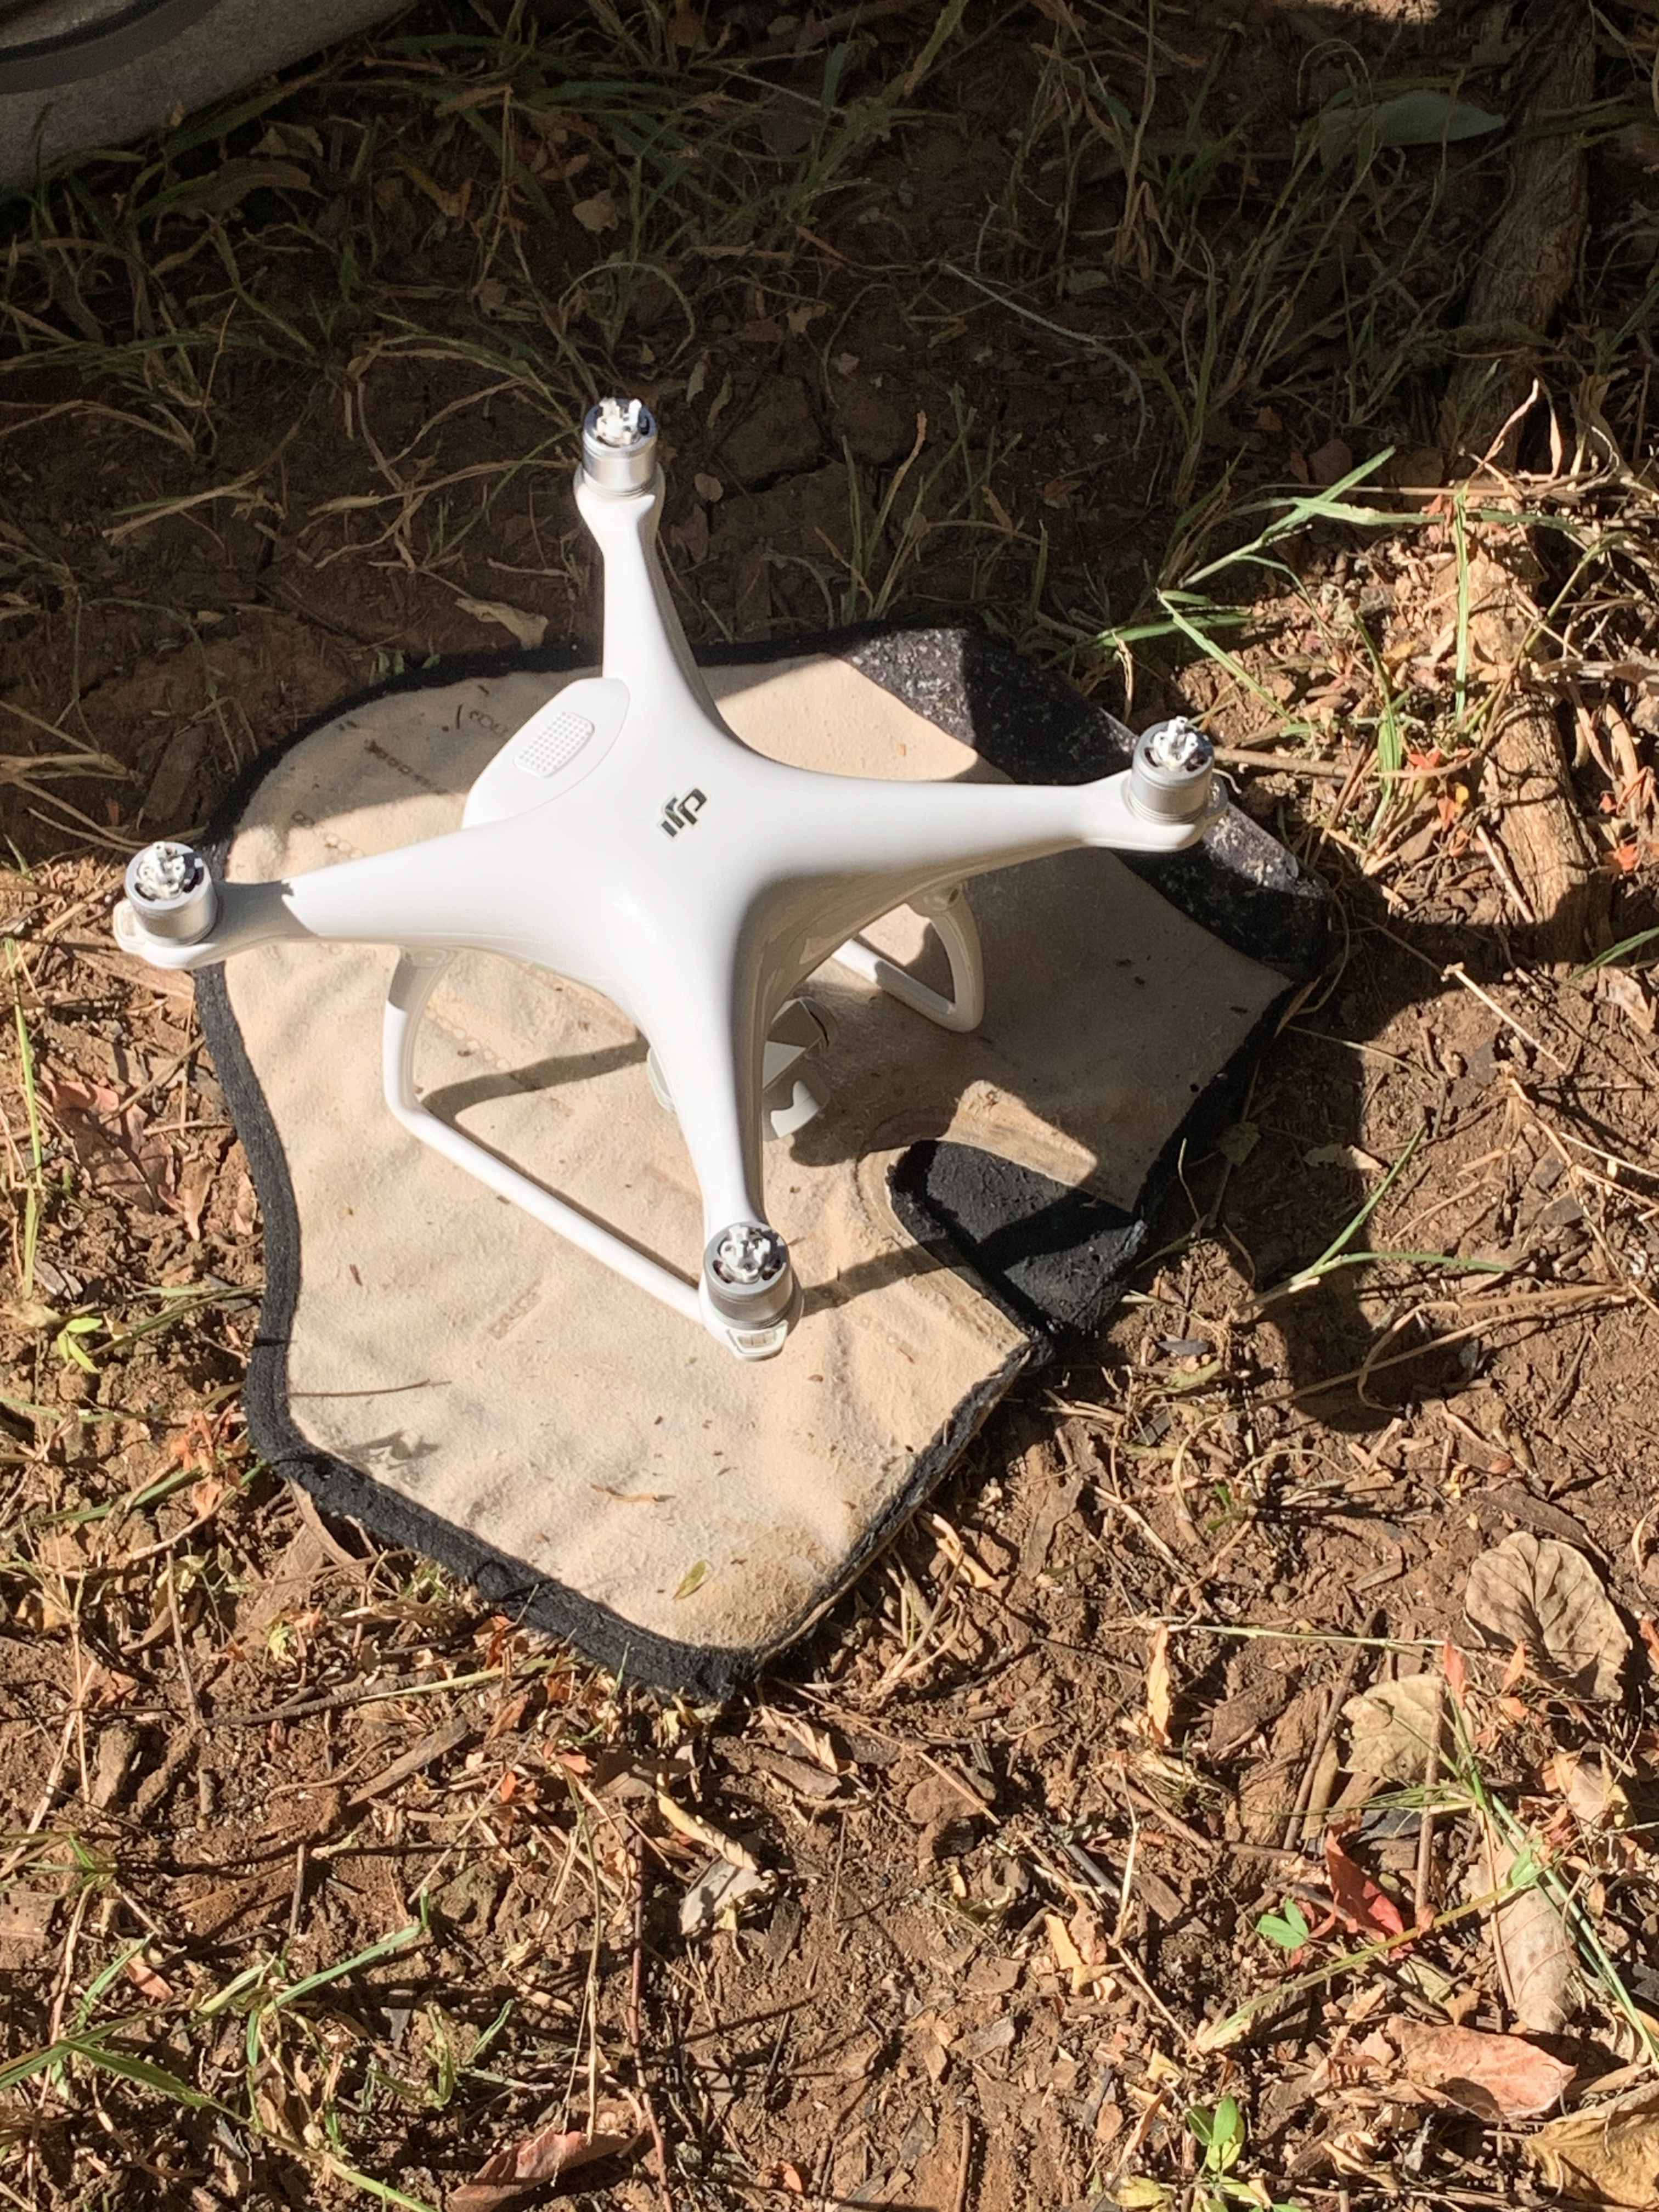
\includegraphics[height=8cm, keepaspectratio]{img/Visitas tecnicas/phantom 4.png}
    \caption{ Drone modelo Phantom 4, utilizado \\ para as capturas das imagens.\\
        \textbf{Fonte:} Acervo pessoal do Ramon Almeida.}
    \label{fig:phantom 4}   
    \end{minipage}
    \hspace{1cm} % Espaço fixo de 0.5cm entre as figuras
    % Segunda figura
    \begin{minipage}{0.45\textwidth} % Reduzi a largura para 45%
        \centering
        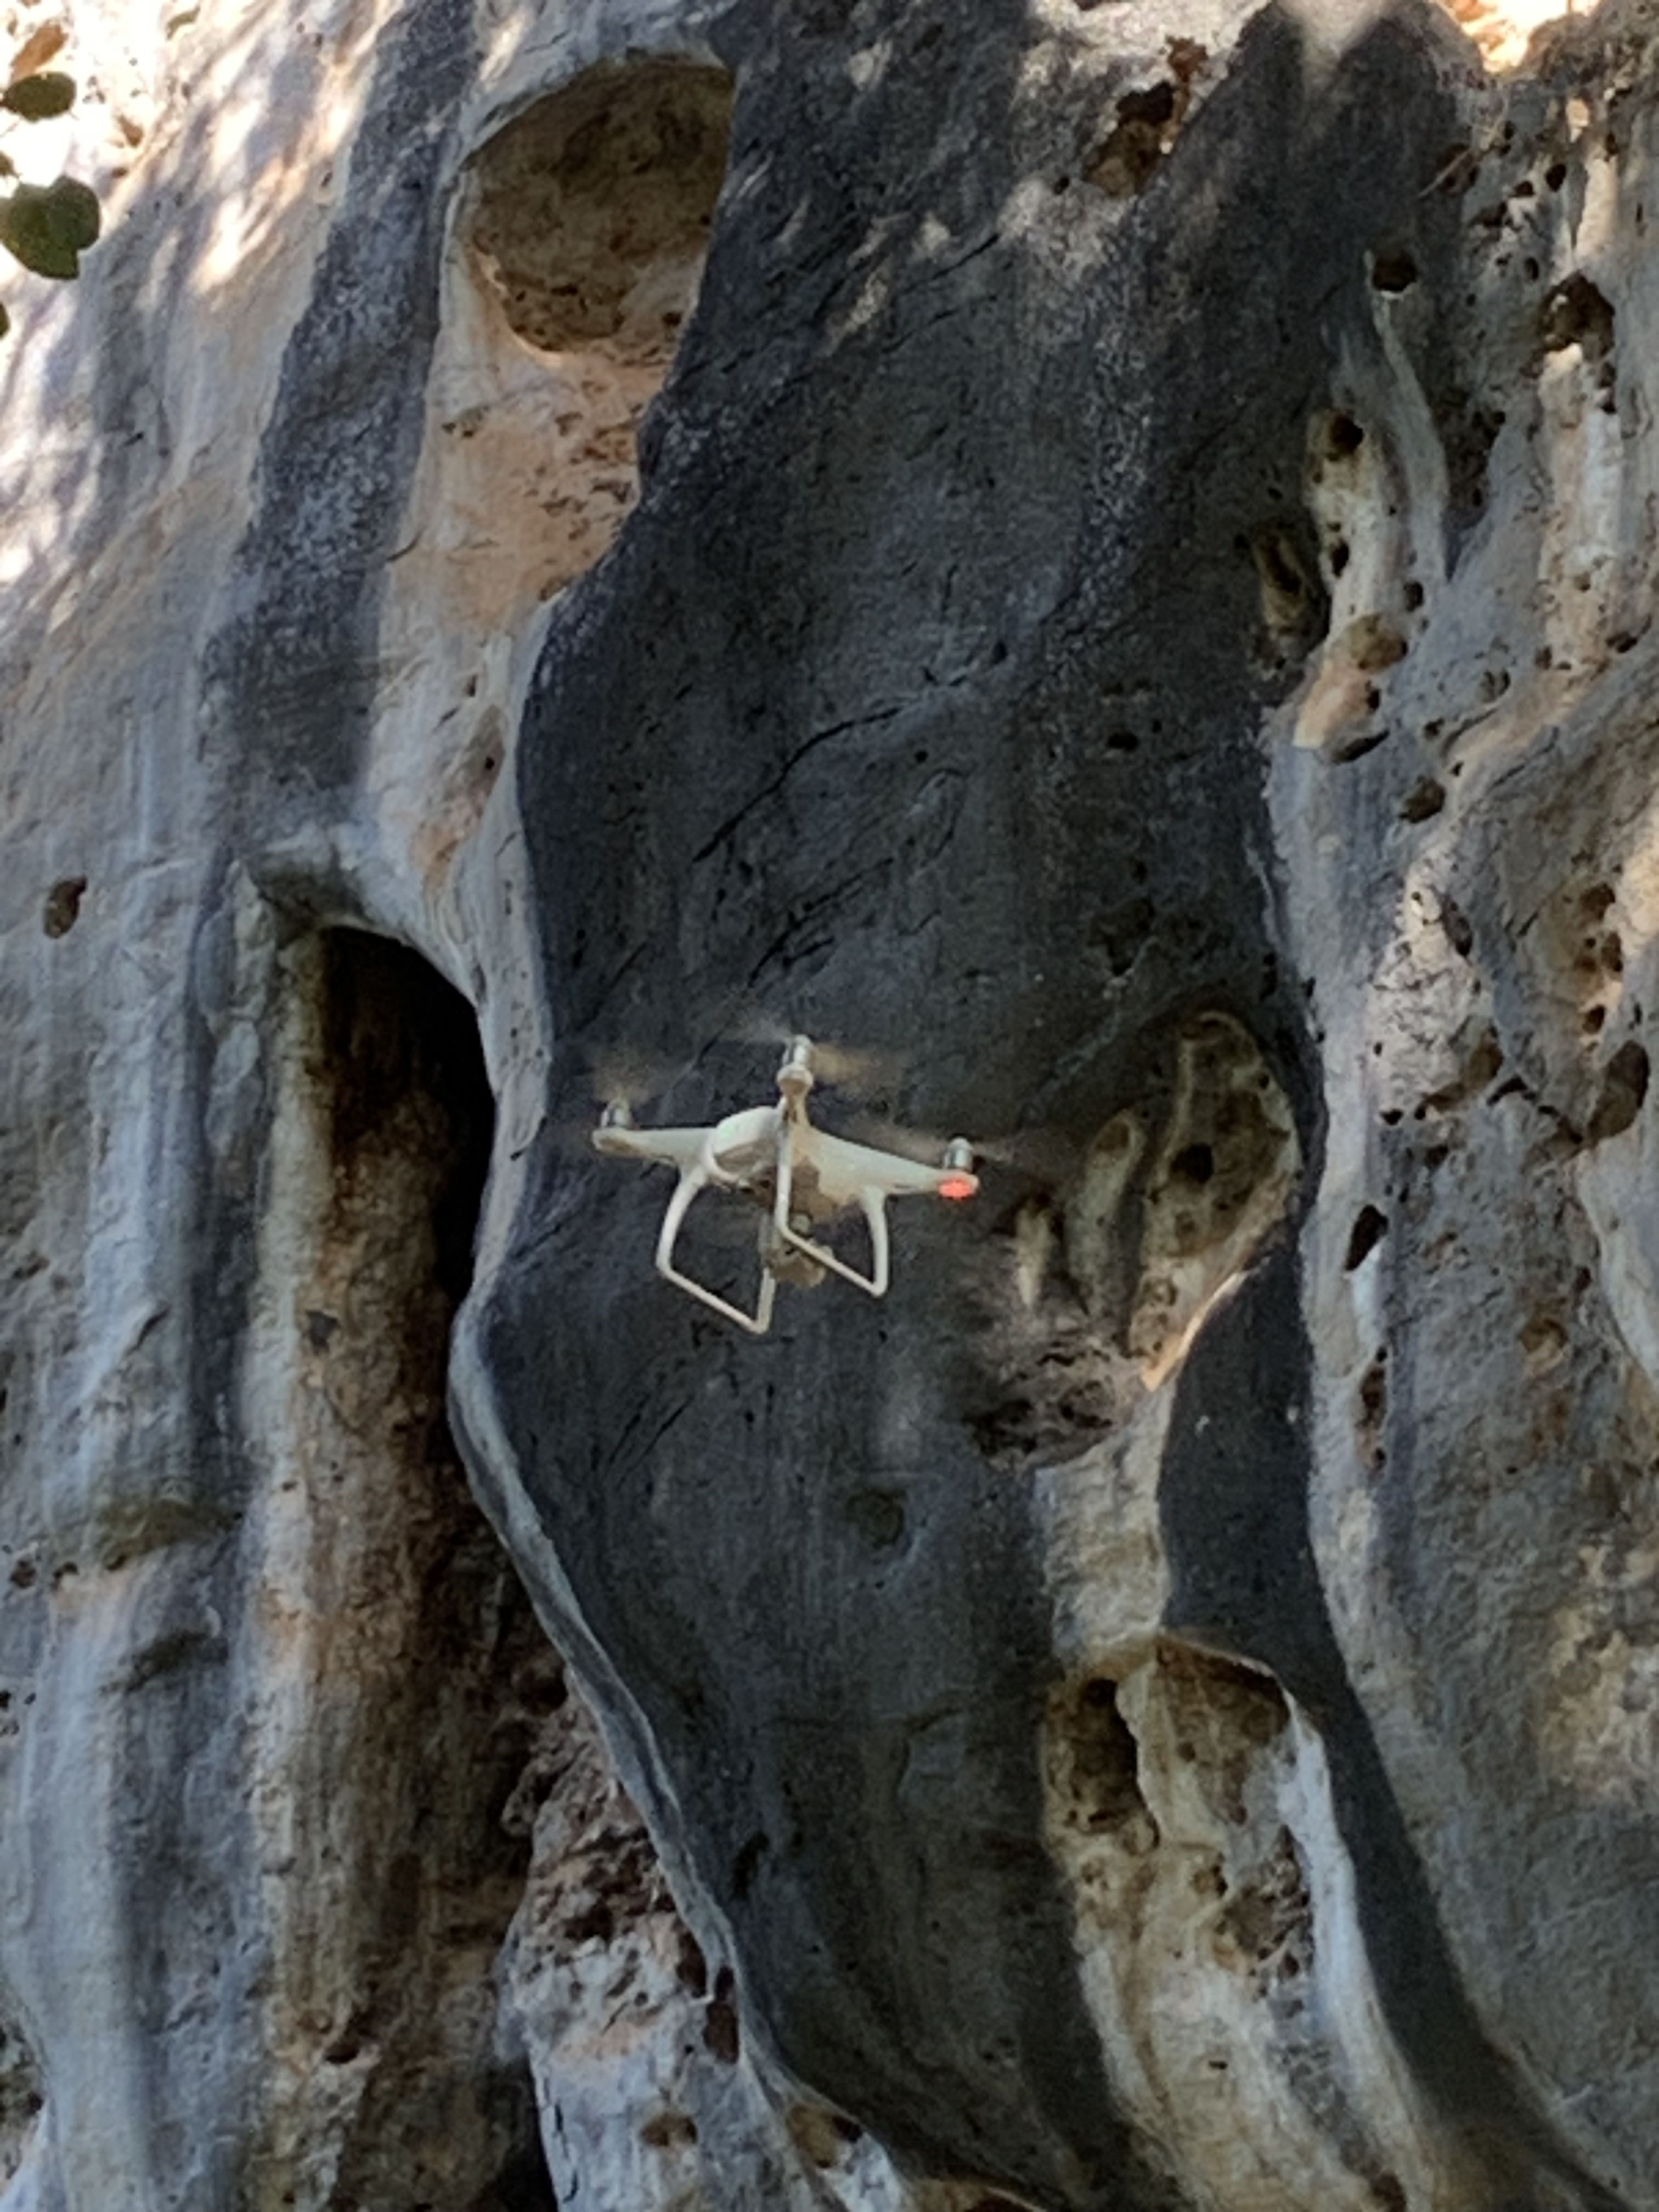
\includegraphics[height=8cm, keepaspectratio]{img/Visitas tecnicas/drone voando.png}
        \caption{Processo de captura de imagens com o \\ drone no exterior da caverna.\\
            \textbf{Fonte:} Acervo pessoal do professor Edson Borges.}
        \label{fig:drone voando}
    \end{minipage}
\end{figure}

\begin{figure}[H]
    \centering
        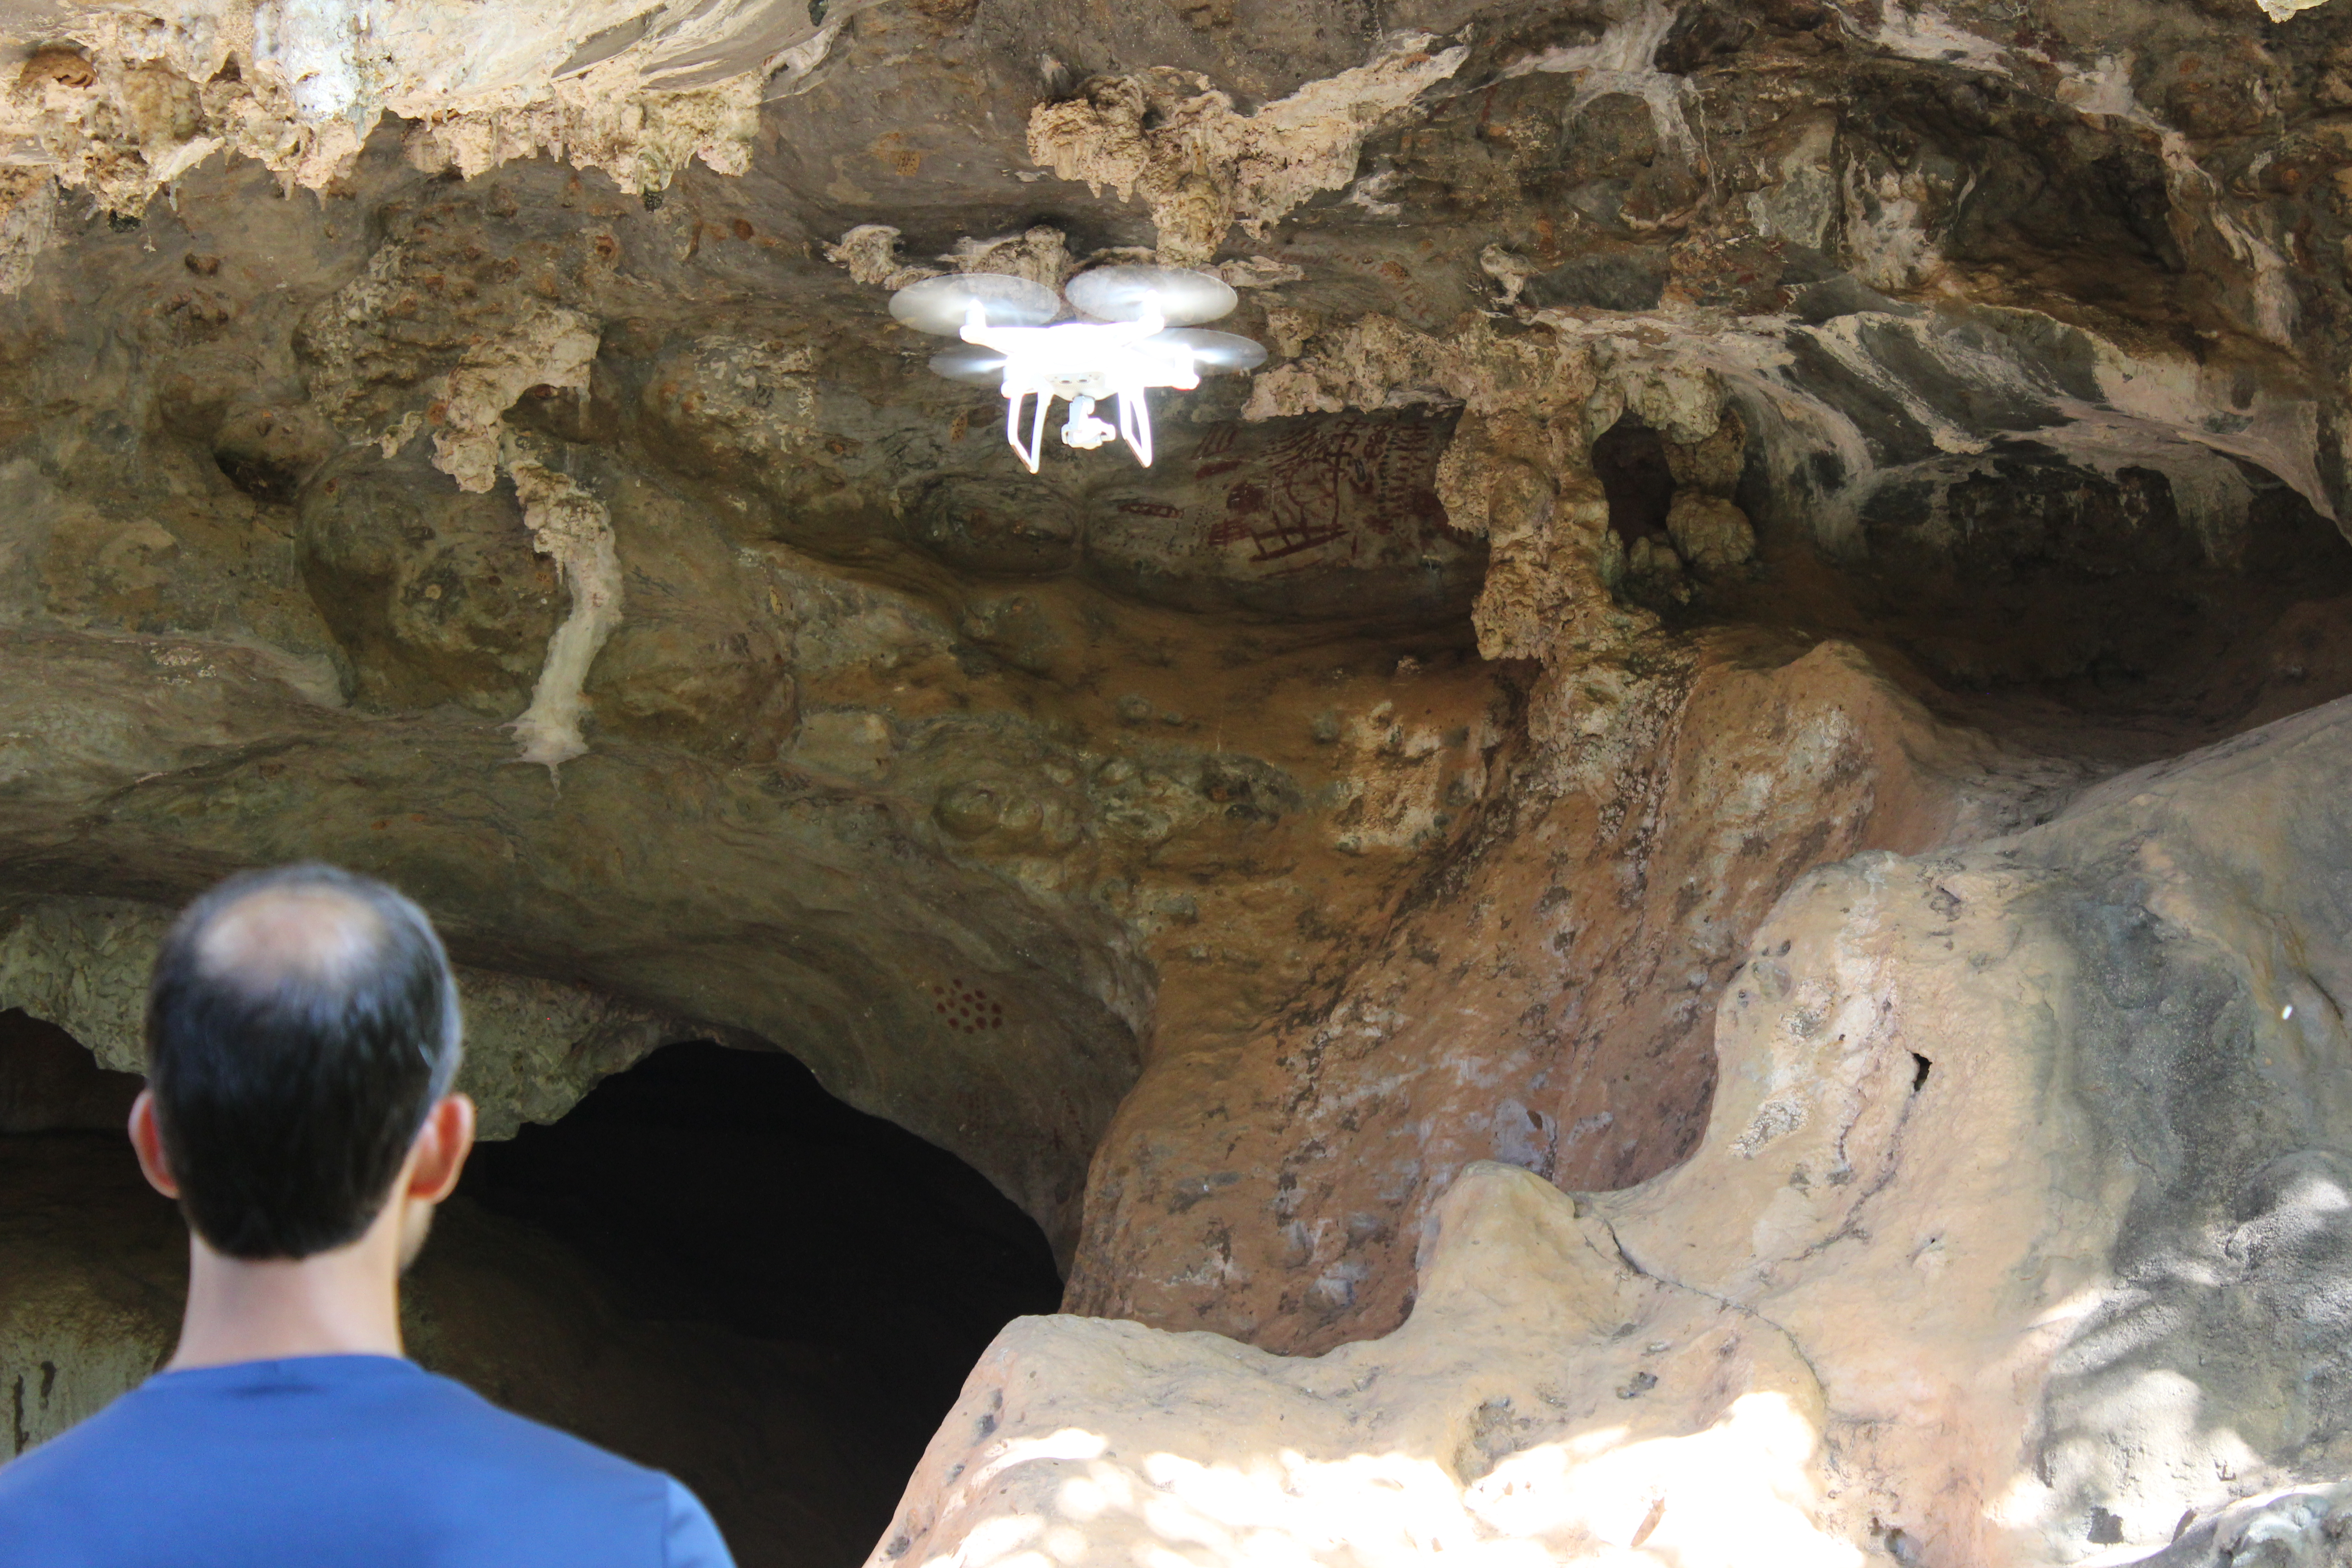
\includegraphics[height=8cm, keepaspectratio]{img/Visitas tecnicas/drone dentro da caverna.jpg}
        \caption{Processo de captura de imagens com o drone \\
        no interior da caverna. \\
            \textbf{Fonte:} Acervo pessoal do Ramon Almeida.}
        \label{fig:drone dentro da caverna}
\end{figure}

 Ao todo foram capturadas 1.493 imagens cobrindo diferentes ângulos do sítio arqueológico. Dessas fotos, 1018 foram selecionadas e as outras foram removidas por conter ruídos, desfoque ou má qualidade que poderiam atrapalhar o processo seguinte (Figura \ref{fig:fotos tiradas}).

\begin{figure}[H]
    \centering
    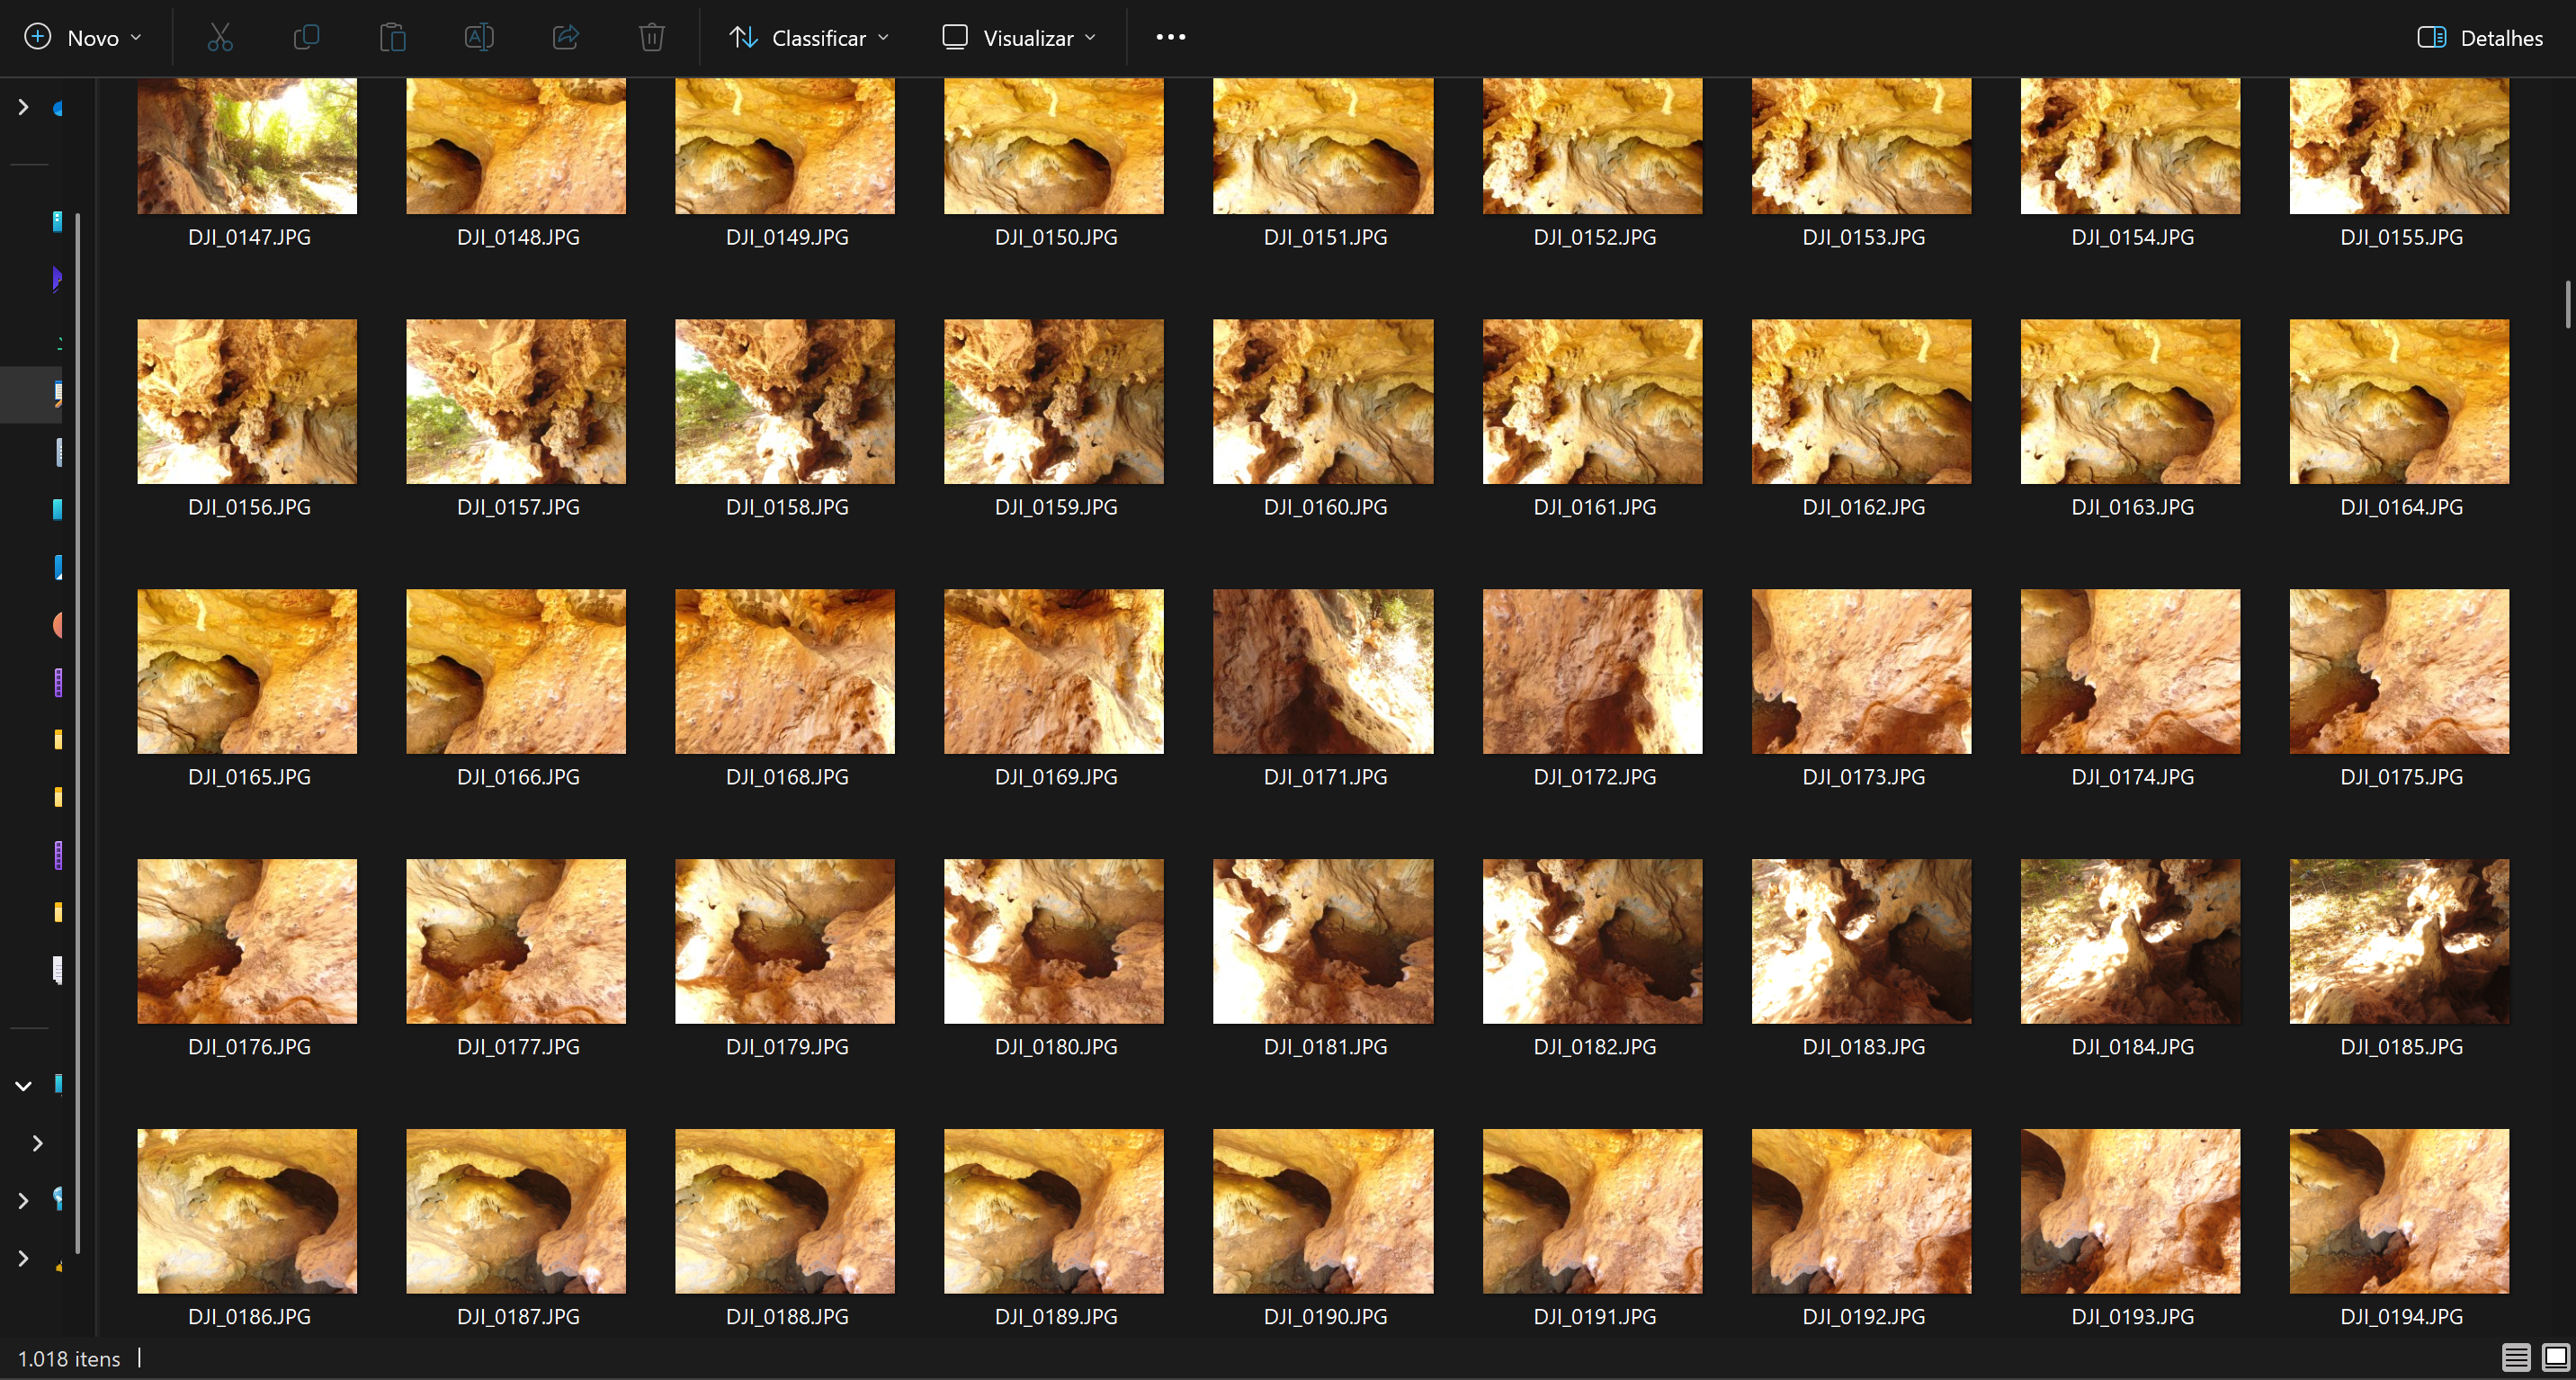
\includegraphics[height=8cm, keepaspectratio]{img/reality e fotogrametria processo/imagens capturas.png}
    \caption{Fotografias capturadas com superposição de 70\%.\\
        \textbf{Fonte:} Elaborado pelo autor.}
    \label{fig:fotos tiradas}   
\end{figure}

    \subsection{Processamento no Reality Capture para reconstrução fotogramétrica}
    \begin{enumerate}
\item \textbf{Alinhamento das Fotos} \\
Com as fotos devidamente selecionadas pôde-se seguir para a etapa de alinhamento, que ocorre no software Reality Capture. O software identifica pontos correspondentes nas imagens e calcula suas posições espaciais relativas (Figura \ref{fig:alinhamento}). Este processo resulta na criação de uma nuvem de pontos esparsa, que representa os principais elementos da cena. 
A partir da nuvem de pontos esparsa, o software gera uma nuvem de pontos densa (Figura \ref{fig:nuvem de pontos}), que contém uma quantidade significativamente maior de pontos e oferece maior detalhamento. Esta etapa é computacionalmente intensiva e depende da qualidade das imagens de entrada.

\begin{figure}[H]
    \centering
        \centering
        \includegraphics[height=8cm, keepaspectratio]{img/reality e fotogrametria processo/cameras alinhamento.png}
        \caption{Alinhamento das imagens pelo software Reality Capture. \\
            \textbf{Fonte:} Elaborado pelo autor.}
        \label{fig:alinhamento}
\end{figure}

\begin{figure}[H]
        \centering
        \includegraphics[height=8cm, keepaspectratio]{img/reality e fotogrametria processo/primeiro modelo componente.png}
        \caption{Nuvem de pontos densa. \\
            \textbf{Fonte:} Elaborado pelo autor.}
        \label{fig:nuvem de pontos}
\end{figure}


\item \textbf{Filtragem e Recorte} \\
Para eliminar pontos indesejados, como vegetação ou objetos móveis, foi realizada uma filtragem manual iterativa. Esta etapa é essencial para garantir que apenas os elementos relevantes sejam incluídos no modelo final.
\begin{figure}[H]
        \centering
        \includegraphics[height=8cm, keepaspectratio]{img/reality e fotogrametria processo/Criação de nuvem de pontos.png}
        \caption{Identificação dos pontos indesejados para filtragem. \\
            \textbf{Fonte:} Elaborado pelo autor.}
        \label{fig:filtragem}
\end{figure}

\item \textbf{Criação do Modelo 3D} \\
Com base na nuvem de pontos densa filtrada, o software gerou a malha poligonal do modelo 3D, como mostra a Figura \ref{fig:modelo 3D solido}. O modelo inicial continha 102 milhões de polígonos, resultando em um nível de detalhe extremamente alto, mas também em um arquivo muito pesado.
\begin{figure}[H]
        \centering
        \includegraphics[height=8cm, keepaspectratio]{img/reality e fotogrametria processo/modelo solido e foto.png}
        \caption{Identificação dos pontos indesejados para filtragem. \\
            \textbf{Fonte:} Elaborado pelo autor.}
        \label{fig:modelo 3D solido}
\end{figure}

\item \textbf{Texturização} \\
O processo de texturização atribuiu cores e detalhes visuais à malha poligonal, utilizando informações das imagens originais. A textura gerada foi de alta qualidade, refletindo fielmente as características do ambiente capturado (Figura \ref{fig:texturizado}). Com esse modelo as figuras pré-históricas no interior da gruta ficaram nítidas e altamente visíveis, como mostra a Figura \ref{fig:interior}.

\begin{figure}[H]
        \centering
        \includegraphics[height=8cm, keepaspectratio]{img/reality e fotogrametria processo/102M textura.png}
        \caption{Modelo texturizado de alta qualidade com 102 milhões de polígonos, parte exterior. \\
            \textbf{Fonte:} Elaborado pelo autor.}
        \label{fig:texturizado}
\end{figure}
\begin{figure}[H]
        \centering
        \includegraphics[height=8cm, keepaspectratio]{img/reality e fotogrametria processo/interior.png}
        \caption{Modelo texturizado de alta qualidade com 102 milhões de polígonos, parte interior. \\
            \textbf{Fonte:} Elaborado pelo autor.}
        \label{fig:interior}
\end{figure}
\end{enumerate}
    \section{Simplificação do Modelo 3D, garantindo compatibilidade com a Unreal Engine (RFA001).}
  
Devido ao tamanho do modelo inicial (102 milhões de polígonos), foi necessário realizar um processo de simplificação para torná-lo mais leve e compatível para uso em softwares como a Unreal Engine, que suporta bem até 5 milhões de polígonos. A malha foi reduzida consideravelmente tornando-o mais leve, porém a qualidade ficou muito ruim deixando os desenhos praticamete apagados, como mostra a Figura \ref{fig:modelo ruim}

\begin{figure}[H]
    \centering
    % Primeira figura
    \begin{minipage}{0.45\textwidth} % Reduzi a largura para 45%
        \centering
        \includegraphics[height=5cm, keepaspectratio]{img/reality e fotogrametria processo/modelo ruim.png}
        \caption{Modelo simplificado com 5 milhões \\ de polígonos. Desenho apagado. \\
            \textbf{Fonte:} Elaborado pelo autor.}
        \label{fig:modelo ruim}
    \end{minipage}
    \hspace{1cm} % Espaço fixo de 0.5cm entre as figuras
    % Segunda figura
    \begin{minipage}{0.45\textwidth} % Reduzi a largura para 45%
        \centering
        \includegraphics[height=5cm, keepaspectratio]{img/reality e fotogrametria processo/desenho bom retroprojeção.png}
        \caption{Modelo simplificado com reprojeção \\ de textura. \\
            \textbf{Fonte:} Elaborado pelo autor.}
        \label{fig:desenho bom}
    \end{minipage}
\end{figure}

  \section{Reprojeção de textura do modelo de alta resolução para o modelo simplificado, mantendo a qualidade visual.} 
  
Para manter a qualidade visual do modelo simplificado, foi aplicada a técnica de reprojeção de textura \ref{fig:desenho bom}. Essa técnica permite utilizar a textura do modelo original de alta qualidade no modelo simplificado, resultando em um equilíbrio ideal entre detalhamento visual e peso computacional. Primeiro é feito o processo de \textit{unwrap}, que pode ser traduzido como "desdobramento UV" ou "mapeamento UV" (Figura \ref{fig:unwrap}). Esta etapa minimiza distorções e sobreposições, garantindo que a textura se encaixe ao objeto 3D de forma realística, facilitando a transposição de texturas de um modelo para o outro. 
\begin{figure}[H]
        \centering
        \includegraphics[height=8cm, keepaspectratio]{img/reality e fotogrametria processo/unwrap.png}
        \caption{Processo de Mapeamento UV. \\
            \textbf{Fonte:} Elaborado pelo autor.}
        \label{fig:unwrap}
\end{figure}

Todo o processo no Reality Capture é demorado e cada etapa pode consumir várias horas. Um dos processos mais rápidos foi o de reprojeção de textura que demorou cerca de apenas 2 horas utilizando um Galaxybook 4 ultra com 32 Gigas de memória RAM, placa de Vídeo NVIDIA 4070 e processador Intel(R) Core(TM) Ultra 9 185H   2.50 GHz com 22 núcleos. Na Figura \ref{fig:reprojecao tempo} pode ser vista uma captura de tela do software processando a reprojeção.
\begin{figure}[H]
        \centering
        \includegraphics[height=8cm, keepaspectratio]{img/reality e fotogrametria processo/reprojeção.png}
        \caption{Processamento da reprojeção de textura. \\
            \textbf{Fonte:} Elaborado pelo autor.}
        \label{fig:reprojecao tempo}
\end{figure}


\end{enumerate}
\subsection{Considerações Finais do Ciclo 1}
O processo de fotogrametria no Reality Capture demonstrou ser uma ferramenta poderosa para a geração de modelos 3D detalhados. A combinação de técnicas como a simplificação de malhas e a reprojeção de textura permitiu criar modelos otimizados para uso em softwares como a Unreal Engine, mantendo alta qualidade visual. Este fluxo de trabalho é essencial para aplicações em um ambiente virtual, a qual é a próxima etapa.

\section{Ciclo 2: Construção do Ambiente Virtual na Unreal Engine}
\label{sec:ciclo2_unreal}
A escolha da plataforma Unreal Engine 5.4 para a criação do ambiente virtual 3D se justifica pela sua capacidade de gerar experiências imersivas e interativas. O Unreal Engine é um motor de criação de jogos amplamente utilizado na indústria de jogos, cinema e arquitetura. A plataforma oferece recursos como simulação de luz, movimentações de câmera e personagens, e a possibilidade de interagir com os elementos do ambiente, tornando o ambiente virtual 3D mais realista e envolvente \citep{silva2022realidade}.

\textbf{Objetivo}: Criar um ambiente virtual interativo e imersivo.

\textbf{Processo}:
\begin{itemize}
    \item Importação do modelo 3D para a Unreal Engine.
    \item Aplicação de texturas, iluminação e configurações de física.
    \item Implementação da navegação do usuário e interações.
\end{itemize}

\section{Ciclo 3: Prototipação do Novo Site}
\label{sec:ciclo3_prototipacao}

\textbf{Objetivo}: Criar um protótipo de alta fidelidade para o site.

\textbf{Processo}:
\begin{itemize}
    \item Criação de uma identidade visual
    \item Definição da arquitetura da informação e wireframes.
    \item Desenvolvimento do protótipo no Figma.
    \item Validação do design com stakeholders.
\end{itemize}

\begin{figure}[H]
    \centering
    \includegraphics[height=8cm, keepaspectratio]{img/Protótipo/logo.png}
    \caption{ Logo do site Arqueologia Formosa inspirada nos pictoglifos e rochas da Lapa da Pedra. \\
        \textbf{Fonte:} Elaborado pelo autor.}
    \label{fig:logo_arqueologia_formosa}
\end{figure}

\begin{figure}[H]
    \centering
    \includegraphics[height=6cm, keepaspectratio]{img/Protótipo/inspiração.png}
    \caption{ Inspirações de outros sites de arqueologia, sites com boa estética, \\ paleta de cores ou forma atrativa. \\
        \textbf{Fonte:} Elaborado pelo autor.}
    \label{fig:inpirações}
\end{figure}

\begin{figure}[H]
    \centering
    \begin{minipage}[b]{0.48\textwidth}
        \centering
        \includegraphics[height=8cm, keepaspectratio]{img/Protótipo/wireframes.png}
        \caption{Wireframes de baixa fidelidade no Figma. \\
            \textbf{Fonte:} Elaborado pelo autor.}
        \label{fig:wireframes}
    \end{minipage}
    \hfill
    \begin{minipage}[b]{0.48\textwidth}
        \centering
        \includegraphics[height=8cm, keepaspectratio]{img/Protótipo/wireframe.png}
        \caption{Wireframe de baixa fidelidade no Figma. \\
            \textbf{Fonte:} Elaborado pelo autor.}
        \label{fig:wireframe}
    \end{minipage}
\end{figure}

\begin{figure}[H]
    \centering
    \includegraphics[height=8cm, keepaspectratio]{img/Protótipo/alta fidelidade.png}
    \caption{ Protótipos de Alta Fidelidade das telas principais no Figma. \\
        \textbf{Fonte:} Elaborado pelo autor.}
    \label{fig:prototipo_alta_fidelidade}
\end{figure}

\begin{figure}[H]
    \centering
    \includegraphics[height=20cm, keepaspectratio]{img/Protótipo/prototipo alta fidelidade toca da onça.png}
    \caption{ Protótipos de Alta Fidelidade das telas principais no Figma. \\
        \textbf{Fonte:} Elaborado pelo autor.}
    \label{fig:prototipo_alta_fidelidade}
\end{figure}


\begin{figure}[H]
    \centering
    \begin{minipage}[b]{0.48\textwidth}
        \centering
        \includegraphics[height=22cm, keepaspectratio]{img/Protótipo/prototipo alta fidelidade toca da onça.png}
        \caption{Wireframes de baixa fidelidade no Figma. \\
            \textbf{Fonte:} Elaborado pelo autor.}
        \label{fig:wireframes}
    \end{minipage}
    \hfill
    \begin{minipage}[b]{0.48\textwidth}
        \centering
        \includegraphics[height=24cm, keepaspectratio]{img/Protótipo/prototipo alta fidelidade toca da onça.png}
        \caption{Wireframe de baixa fidelidade no Figma. \\
            \textbf{Fonte:} Elaborado pelo autor.}
        \label{fig:wireframe}
    \end{minipage}
\end{figure}

\section{Ciclo 4: Desenvolvimento do Novo Site}
\label{sec:ciclo4_desenvolvimento}

\textbf{Objetivo}: Implementar o site final baseado no protótipo validado.

\textbf{Processo}:
\begin{itemize}
    \item Configuração do ambiente \textit{JAMstack} com Next.js, Sanity e Schema UI.
    \item Implementação de páginas e funcionalidades.
    \item Otimizações de performance e SEO.
    \item Testes e ajustes finais.
\end{itemize}

\textbf{Imagens e Evidências}:
Adicionar prints das telas implementadas, código relevante e testes realizados.

\section{Avaliação e Testes}
\label{sec:avaliacao_testes}

\textbf{Objetivo}: Garantir que a solução atenda aos requisitos definidos.

\textbf{Processo}:
\begin{itemize}
    \item Testes de usabilidade.
    \item Validação heurística.
    \item Avaliação de performance e responsividade.
\end{itemize}

\textbf{Imagens e Evidências}:
Adicionar capturas de relatórios de testes, feedbacks coletados e ajustes realizados.

\section{Publicação e Deploy}
\label{sec:publicacao_deploy}

\textbf{Objetivo}: Tornar o projeto acessível ao público.

\textbf{Processo}:
\begin{itemize}
    \item Deploy na Vercel e disponibilização pública do site (Figura \ref{fig:deploy_vercel}). 
\begin{figure}[H]
    \centering
    \includegraphics[height=8cm, keepaspectratio]{img/Deploy/deploy_vercel.png}
    \caption{ Captura de tela do processo de deploy na vercel com esteira CI/CD integrada. \\
        \textbf{Fonte:} Elaborado pelo autor.}
    \label{fig:deploy_vercel}
\end{figure}

    \item Registro de domínio pelo \href{www.registro.br}{Registro.br}, que é o departamento do NIC.br responsável pelas atividades de registro e manutenção dos nomes de domínios que usam o .br. Essa escolha garante maior confiabilidade, identidade nacional e melhor indexação nos mecanismos de busca (Figura \ref{fig:dominio_registro_br}).
\begin{figure}[H]
    \centering
    \includegraphics[height=8cm, keepaspectratio]{img/Deploy/domínio-registro.br.png}
    \caption{ Domínio disponível para compra no site \href{www.registro.br}{Registro.br}. \\
        \textbf{Fonte:} Elaborado pelo autor.}
    \label{fig:dominio_registro_br}
\end{figure}

    \item Configuração de DNS para apontar o domínio para a Vercel (Figura \ref{fig:dns}).
\begin{figure}[H]
    \centering
    \includegraphics[height=8cm, keepaspectratio]{images/dns_config.png}
    \caption{ Configuração de DNS para apontar o domínio para a Vercel. \\
        \textbf{Fonte:} Elaborado pelo autor.}
    \label{fig:dns}
\end{figure}

\end{itemize}



